



\section{Day ahead and real time energy prices}




\section{Characteristics of energy markets}

Ideas: 

\begin{itemize}
	\item Show electricity price variation for market over a 3 year period (Weron, pg 33)
	\item Show autocorrelation function over extended (same) time period
	\item Show periodogram over extended time period
\end{itemize}




See folders "`Electricity pricing"' and "`power markets"'


\begin{figure}[htbp]
	\centering
		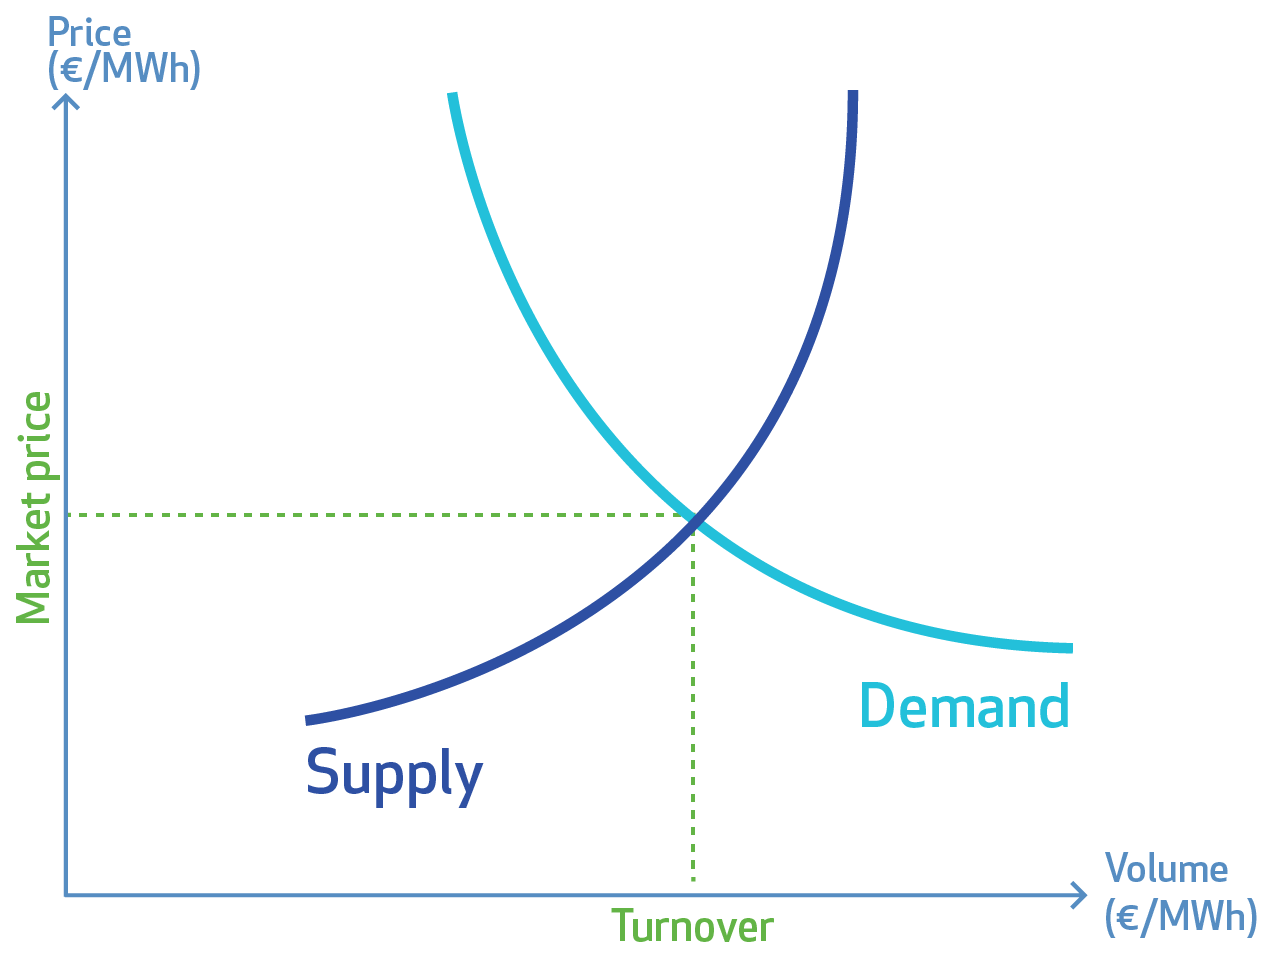
\includegraphics[width=0.5\textwidth]{figures/data_analysis/DA_supply_demand.png}
	\caption{Intersection between supply and demand \cite{nord2014supply}}
	\label{fig:DA_supply_demand}
\end{figure}



In this section different studies of power market characteristics are presented to distinguish features that may be used in building forecasting models. 

\subsection{Stable Modeling of different European Power Markets}

In \cite{mugele2005stable} different European power markets have been investigated to reveal major differences in energy price behaviour. The EEX, Nord Pool Spot and Polish power markets have been evaluated whereby the markets are responsible for the Mid-Europe, Northern Europe and Polish regions respectively. 

As electricity prices depend on energy demand \cite{weron2005forecasting} which changes due to climate conditions (temperature and number of daylight hours) electricity prices exhibit a seasonal component as well (Figure \ref{fig:seasonal_behaviour_of_eex_prices}). 

\begin{figure}[htbp]
	\centering
		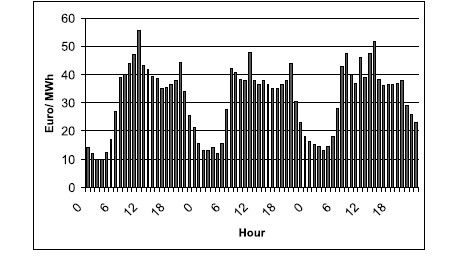
\includegraphics{figures/state_of_the_art/seasonal_behaviour_of_eex_prices.PNG}
	\caption{EEX - hourly spot prices \cite{mugele2005stable}}
	\label{fig:seasonal_behaviour_of_eex_prices}
\end{figure}

The daily seasonality for hourly spot prices at EEX (Figure \ref{fig:seasonal_behaviour_of_eex_prices}) can be clearly spotted where prices 
start rising at 6 a.m.~to 8 a.m.~and begin to fall at 6 p.m.~to 8 p.m. Daily variations of prices are caused by reduced electricity demand and power consumption at nights. 

The main differences between electricity power markets and other financial markets are price volatility, mean reversion and price jumps or "`spikes"'. Volatility is high as generated electricity cannot be stored but has to be delivered at once which might lead to high prices due to transmission congestion or surges in demand. It's impact can be reduced by applying logarithmic transformations to input data \cite{weron2005forecasting}. 

Energy prices experience strong mean reversion which denotes the characteristic that prices return to their mean levels after an increase in prices. In addition price spikes may appear where prices can increase tenfold from one hour to the next. To mitigate these spikes they may be averaged out in a data preprocessing step. 

Even though price seasonality and trend seem to be stable over a short time range (Figure \ref{fig:seasonal_behaviour_of_eex_prices}) they can show significant fluctuations over a longer time range. In \cite{mugele2005stable} data related to each examined energy market was fitted to a stable Paretian distribution as well as a normal distribution. The result showed that mature markets as EEX or Nord Pool Spot exhibit high volatility, heavy tails, high kurtosis and asymmetrics in the energy price data which was best modeled by the Paretian distribution. In contrast the Gielda Energii SA market in Poland shows a much more stable energy price behavior which can be modeled by a Gaussian distribution. 

The variation in energy price levels for the two power markets EEX and Nord Pool Spot are shown in Figures \ref{fig:EEX_levels} and \ref{fig:NordPool_levels}.

\begin{figure}[!htbp]
  \centering
  \begin{minipage}[b]{0.4\textwidth}
    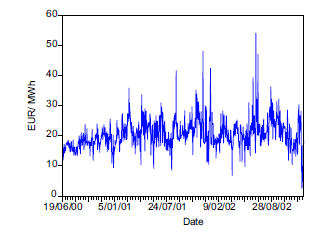
\includegraphics[width=\textwidth]{figures/state_of_the_art/EEX_levels.PNG}
    \caption{EEX levels \cite{mugele2005stable}}
		\label{fig:EEX_levels}
  \end{minipage}
  \hfill
  \begin{minipage}[b]{0.4\textwidth}
    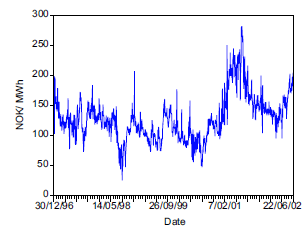
\includegraphics[width=\textwidth]{figures/state_of_the_art/NordPool_levels.PNG}
    \caption{Nord Pool levels \cite{mugele2005stable}}
		\label{fig:NordPool_levels}
  \end{minipage}
\end{figure}

Even though the figures above show neither the same time ranges nor the same scale (150 NOK equal to about 20 Euros in 2002) it is clearly visible that both energy price levels and amount of price variation can be very different across power markets. 

%This shows that it is important to investigate energy price characteristics from power markets to accurately model market prices. 



%
%\subsection{Electricity markets and pricing}
%
%In wholesale energy markets different pricing and bidding models can be used. Currently the two most common price evaluation strategies are day-ahead and real-time pricing strategies. 
%
%\subsubsection{Bidding strategies}
%
%In \cite{tierney2008uniform} two different bidding strategies are discussed, uniform pricing and pay-as-bid auctions. In the uniform pricing model the market clearing price is determined by collecting the marginal prices from all suppliers and taking the maximum price from this collection. Conversely, in pay-as-bid auctions a supplier gets paid based on its actual bid. 
%The second approach may seem beneficial from the customer's point of view since suppliers may set individual prices which enables competition within the market. 
%However studies show that in this pricing scheme suppliers set their prices at the maximum possible level to be comparable to other suppliers and keep their customers. On the other hand the uniform pricing model provides a uniform clearing price which is valid for all participants in the market and customers may trust that suppliers set prices to just satisfy their needs. 


\section{Energy price case study}

In this section the aforementioned characteristics of electricity prices in power markets will be investigated for both day ahead and real time energy price data within a time range of three years. 


\subsection{Electricity market price characteristics}

Through display of energy price time series over an extended time range the general behavior of different energy markets can be observed. Day ahead and real time energy price time series have been collected for the years 2012 to 2014 which are displayed in figures \ref{fig:da_energy_markets_2012_2014} and \ref{fig:rt_energy_markets_2012_2014}. 

The title displays the name of the energy market followed by the country abbreviation and an indicator whether this market is a day ahead or real time market (DA or RT). Strongest price variations are experienced in real time markets (figure \ref{fig:rt_energy_markets_2012_2014}) where price spikes of almost 2000 \$/MWh occur. 


\begin{figure}[htbp]
	\centering
		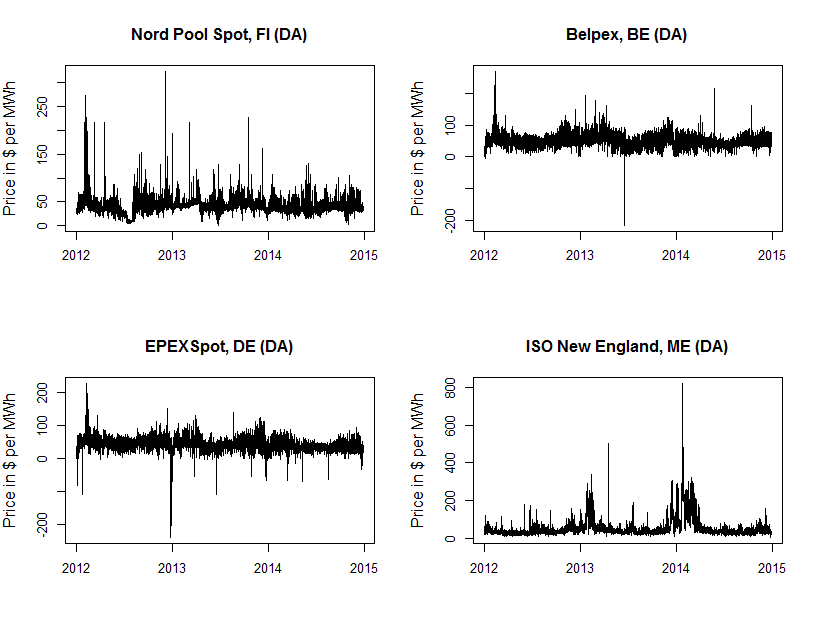
\includegraphics[width=0.8\textwidth]{figures/data_analysis/da_energy_markets_2012_2014.png}
	\caption{Day ahead energy market prices}
	\label{fig:da_energy_markets_2012_2014}
\end{figure}

\begin{figure}[htbp]
	\centering
		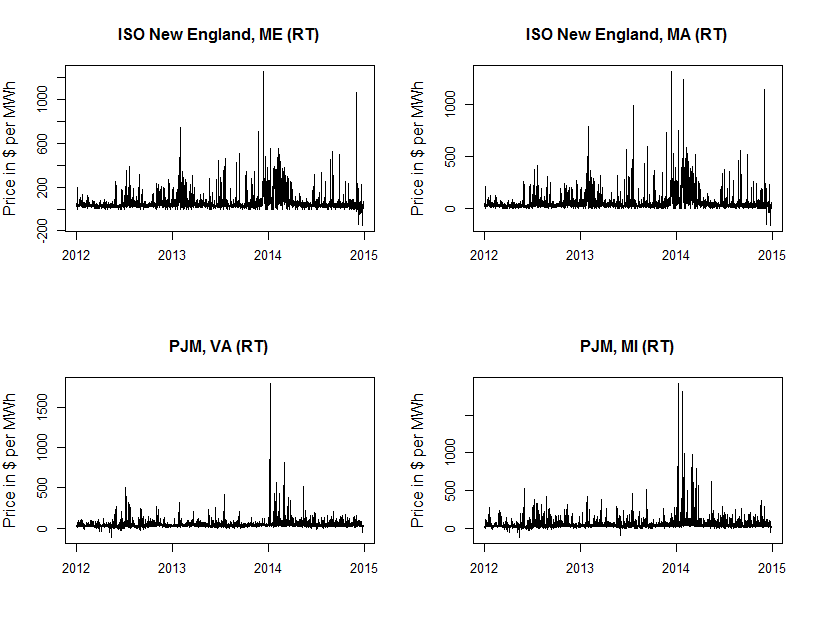
\includegraphics[width=0.8\textwidth]{figures/data_analysis/rt_energy_markets_2012_2014.png}
	\caption{Real time energy market prices}
	\label{fig:rt_energy_markets_2012_2014}
\end{figure}

What can be noted is that markets Belpex and EPEXSpot appear to be the most stable in terms of energy price level and variations except some occasional negative spikes throughout the dataset. The aggregated statistics for each market are outlined in tables \ref{table:day_ahead_market_summary} and \ref{table:real_time_market_summary}. 

The inter quartile range (range between 1st quartile and 3rd quartile) of the market prices lies between 20 \$/MWh and 60 \$/MWh whereas the minimum and maximum values tend to lie far outside this range. Real time markets exhibit significantly greater values for skewness and kurtosis which indicates a higher probability of extreme price spikes. When comparing maximum price values of real time markets to those of day ahead markets this fact is supported as well. 
The stable variability of Belpex and EPEXSpot is also emphasized through a low absolute value for the skewness which indicates an almost symmetrical distribution. In contrast, other markets are heavy tailed and experience far more "`outliers"' indicated by a higher value for skewness. 



%%%%%%%%%%%%%%%%%%%%%%%%%%%%%%%%%%%%%%%%%%%%%%%%%%%%%%
%%%%%%%%%% Skewness and kurtosis explanation %%%%%%%%%
%%%%%%%%%%%%%%%%%%%%%%%%%%%%%%%%%%%%%%%%%%%%%%%%%%%%%%

%Skewness quantifies how symmetrical the distribution is.
%
%•	A symmetrical distribution has a skewness of zero.
%•	An asymmetrical distribution with a long tail to the right (higher values) has a positive skew.
%•	An asymmetrical distribution with a long tail to the left (lower values) has a negative skew.
%•	The skewness is unitless.
%•	Any threshold or rule of thumb is arbitrary, but here is one: If the skewness is greater than 1.0 (or less than -1.0), the skewness is substantial and the distribution is far from symmetrical.
%Kurtosis quantifies whether the shape of the data distribution matches the Gaussian distribution.
%
%•	A Gaussian distribution has a kurtosis of 0.
%•	A flatter distribution has a negative kurtosis,
%•	A distribution more peaked than a Gaussian distribution has a positive kurtosis.
%•	Kurtosis has no units.
%•	The value that Prism reports is sometimes called the excess kurtosis since the expected kurtosis for a Gaussian distribution is 0.0.
%•	An alternative definition of kurtosis is computed by adding 3 to the value reported by Prism. With this definition, a Gaussian distribution is expected to have a kurtosis of 3.0.
%
%http://www.graphpad.com/guides/prism/6/statistics/index.htm?stat_skewness_and_kurtosis.htm


%> xtable(da_statistics)
% latex table generated in R 3.1.1 by xtable 1.8-2 package
% Mon Mar 14 05:40:05 2016
\begin{table}[ht]
\centering
\begin{tabular}{rrrrrrrrr}
  \hline
 & Min & 1st Qu. & Median & Mean & 3rd Qu. & Max & Skew. & Kurt. \\ 
  \hline
NPS, FI (DA) & 1.49 & 33.08 & 39.18 & 40.91 & 46.33 & 324.00 & 3.60 & 40.02 \\ 
  Belpex, BE (DA) & -216.00 & 37.14 & 48.60 & 48.66 & 59.49 & 270.00 & 0.08 & 13.35 \\ 
  EPEXSpot, DE (DA) & -239.70 & 31.20 & 39.34 & 40.73 & 51.16 & 226.80 & -1.06 & 25.29 \\ 
  ISO NE, ME (DA) & 3.00 & 28.94 & 37.18 & 50.78 & 50.41 & 817.70 & 3.62 & 23.62 \\ 
   \hline
\end{tabular}
\caption{Day ahead energy market summary statistics}
\label{table:day_ahead_market_summary}
\end{table}
%> xtable(rt_statistics)
% latex table generated in R 3.1.1 by xtable 1.8-2 package
% Mon Mar 14 05:40:06 2016
\begin{table}[ht]
\centering
\begin{tabular}{rrrrrrrrr}
  \hline
 & Min & 1st Qu. & Median & Mean & 3rd Qu. & Max & Skew. & Kurt. \\ 
  \hline
ISO NE, ME (RT) & -147.00 & 26.42 & 34.83 & 49.21 & 48.90 & 1257.00 & 4.24 & 42.21 \\ 
  ISO NE, MA (RT) & -153.90 & 27.24 & 35.99 & 52.23 & 50.92 & 1310.00 & 4.76 & 48.87 \\ 
  PJM, VA (RT) & -118.60 & 26.33 & 30.34 & 35.85 & 36.93 & 1789.00 & 24.53 & 996.02 \\ 
  PJM, MI (RT) & -120.80 & 27.76 & 32.82 & 43.83 & 41.52 & 1913.00 & 14.12 & 316.98 \\ 
   \hline
\end{tabular}
\caption{Real time energy market summary statistics}
\label{table:real_time_market_summary}
\end{table}


In order to visualize the aforementioned statistical properties histograms have been generated for each market over the whole time range \ref{fig:Histograms_da_2012_2014}, \ref{fig:Histograms_rt_2012_2014}. 

As outlined before the Belpex and EPEXSpot markets exhibit the most stable distribution of prices which is visible in the histograms as these markets show the most symmetric distributions. They exhibit an almost gaussian like distribution whereas other markets are clearly heavy tailed to the right. In order to see the distribution of prices more distinctly the histograms where cut off at 250 \$/MWh to be able to accurately compare the price distributions. 




\begin{figure}[htbp]
	\centering
		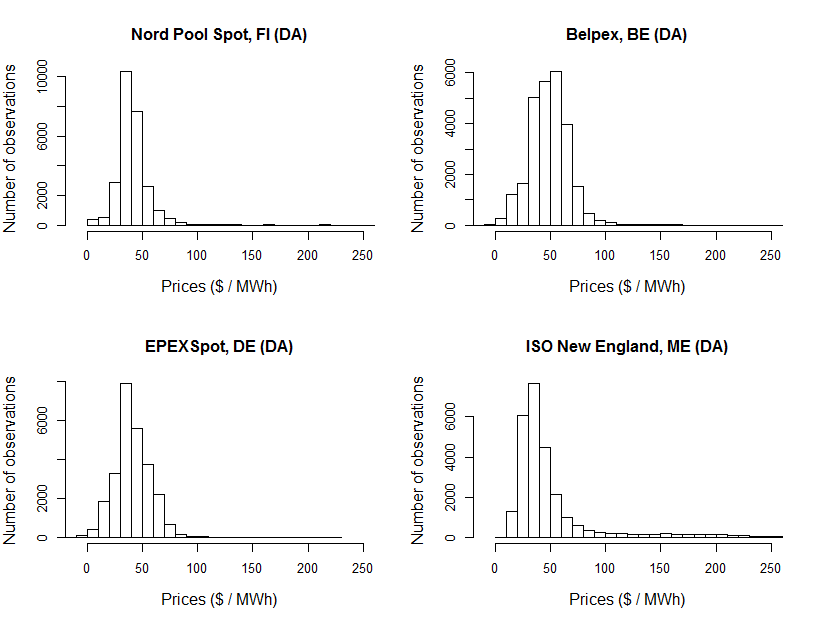
\includegraphics[width=0.8\textwidth]{figures/data_analysis/Histograms_da_2012_2014.png}
	\caption{Histograms of day ahead markets for years 2012 to 2014}
	\label{fig:Histograms_da_2012_2014}
\end{figure}

\begin{figure}[htbp]
	\centering
		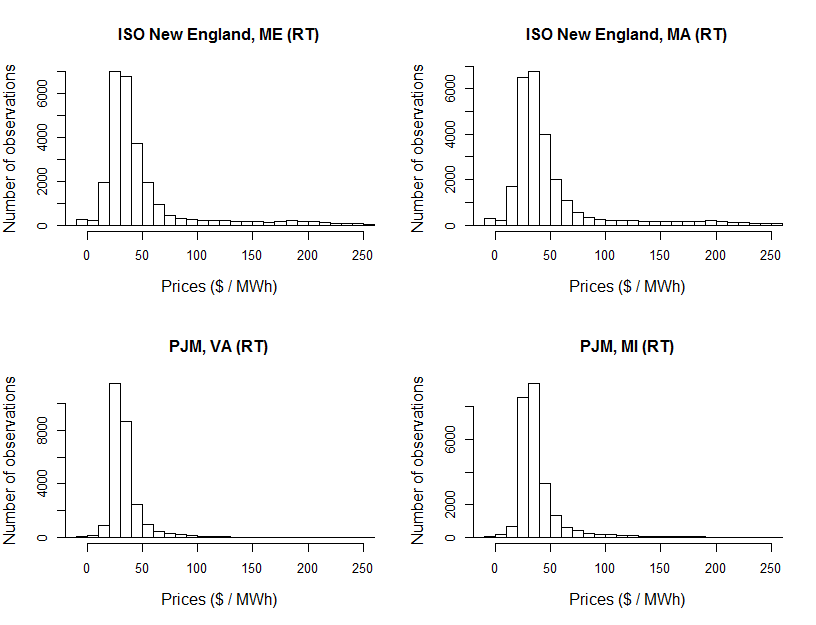
\includegraphics[width=0.8\textwidth]{figures/data_analysis/Histograms_rt_2012_2014.png}
	\caption{Histograms of real time markets for years 2012 to 2014}
	\label{fig:Histograms_rt_2012_2014}
\end{figure}




